\documentclass{ctexart}
\usepackage{EC}
\begin{document}
\section{硒,碲及其化合物}
\subsection{硒,碲的单质}
\subsection{硒,碲的化合物}
\subsubsection{\ce{S,Se,Te}的多原子阳离子}
\paragraph{多硫阳离子}早在1804年,G.F.Bucholz发现将硫溶解在发烟硫酸中可得清澈透亮的溶液.随着发烟硫酸的强度和反应时间不同,溶液可呈黄色,深蓝色或红色(或其中间色).现已得知,在这些溶液中含有\ce{S_n^2+}离子.\\
\indent 硫在惰性溶剂(如\ce{SO2})中极易被\ce{SbF5}或\ce{AsF5}定量氧化为深蓝色的\ce{S8^2+}离子,例如:
\begin{center}
    \ce{S8 + 2AsF5 -> [S8]^2+[AsF6]^-_2 + AsF3}
\end{center}
在前述黄色的溶液中含有\ce{S4^2+},它具有平面正方形的环状结构,理论上具有芳香性.在前述红色的溶液中含有\ce{S_19^2+}.
\paragraph{多硒阳离子}
硫溶于发烟硫酸中得亮色溶液,\ce{Se}与\ce{Te}也有类似的
性质.对非水溶剂范围内的系统研究表明\ce{Se}与\ce{Te}多原子阳离子比\ce{S}的同系物的电正性低,可以用种类更多的强酸制备.下面是\ce{Se}可以发生的典型反应:
\begin{center}
    \ce{4Se + (SO3F)2 ->T[\ce{HSO3F}] [Se4]^2+[SO3F]^-_2}\\
    \ce{Se_4^2+ + 4Se ->T[\ce{HSO3F}] [Se8]^2+}\\
    \ce{Se_8 + 6AsF5 ->T[\ce{SO2}] 2[Se4]^2+[AsF6]^-_2 + 2AsF3}\\
    \ce{Se_8 + 5SbF5 ->T[\ce{SO2}] [Se8]^2+[Sb2F11]^-_2 + SbF3}\\
    \ce{15Se + SeCl4 + 4AlCl3 ->[$250\tccentigrade$] 2[Se8]^2+[AlCl4]^-_2}
\end{center}
\indent \ce{Se4^2+}是黄色的,而\ce{Se8^2+}则是绿色的.后来,通过\ce{SbF5}与过量\ce{Se}在\ce{SO2}中反应,又得到了深红色的\ce{Se10(SbF6)2}.
\paragraph{多碲阳离子}
用上述相似方法可以制备多原子\ce{Te}阳离子.\\
\indent \ce{Te4^2+}是亮红色的,而\ce{Te8^2+}尚未得到.在\ce{AsF3}溶剂中用\ce{AsF5}氧化\ce{Te}可以生成棕色的晶体\ce{[Te6][AsF6]4.2AsF3}:
\begin{center}
    \ce{6Te + 6AsF5 ->T[AsF3] [Te6]^2+[AsF6]^-_4.2AsF3}
\end{center}
\ce{Te6^4+}是三棱柱型的阳离子簇.
\paragraph{\ce{S,Se,Te}的多原子阳离子的结构}
下面给出了前述几种阳离子的立体结构.
\begin{figure}[H]
    \centering
    \subfigure[\ce{X4^2+}$\left(\ce{X}=\ce{S,Se,Te}\right)$的结构]
    {
        \begin{minipage}[b]{.45\linewidth}
            \centering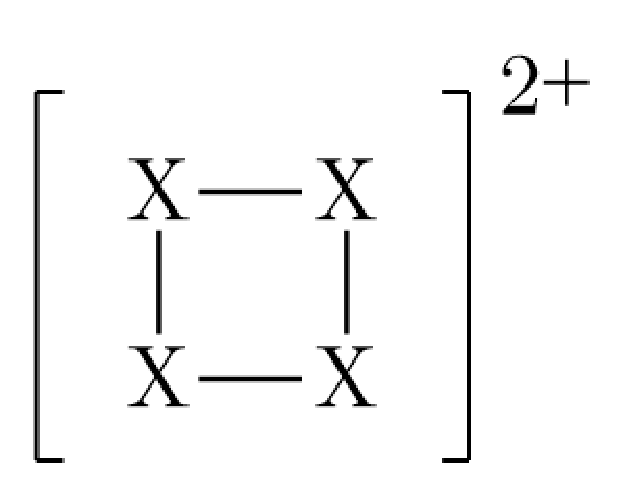
\includegraphics[scale=0.25]{picture/X42+.eps}
        \end{minipage}
    }
    \subfigure[\ce{Te6^4+}的结构]
    {
        \begin{minipage}[b]{.45\linewidth}
            \centering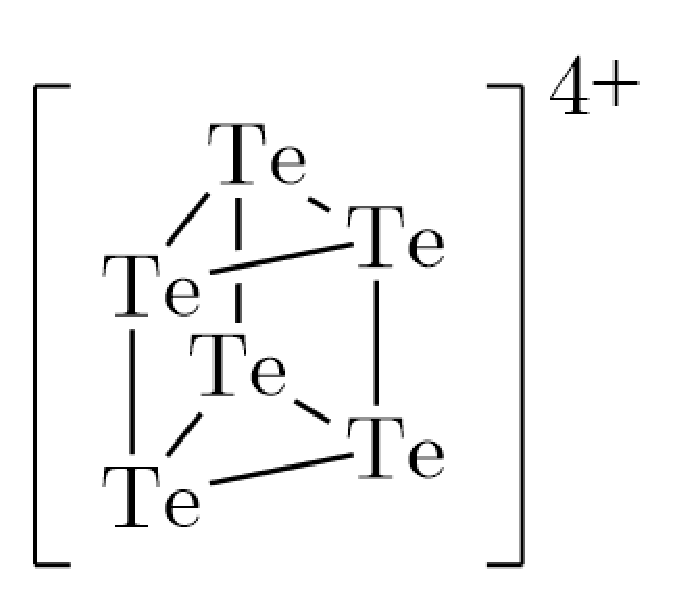
\includegraphics[scale=0.25]{picture/Te64+.eps}
        \end{minipage}
    }
    \caption{部分\ce{S,Se,Te}的多原子阳离子的结构}
\end{figure}
\subsubsection{\ce{Se,Te}的卤化物}
\paragraph{\ce{Te}的低卤化物}
\paragraph{\ce{Se,Te}的四卤化物}
\paragraph{\ce{Se,Te}的六卤化物}
\subsubsection{\ce{Se,Te}的$\mbf{-2}$价化合物}
\begin{substance}[\ce{H2Se}]
    硒化氢,化学式为\ce{H2Se},是无色,有恶臭,有毒的气体,可溶于水,溶解度与\ce{H2S}相近.
\end{substance}
\begin{substance}[\ce{H2Te}]
    碲化氢,化学式为\ce{H2Te},是无色,有恶臭,有毒的气体,可溶于水,溶解度与\ce{H2S}相近.
\end{substance}
\ce{H2Se}(与\ce{H2O}及\ce{H2S}相似)可用相应的单质在$350\tccentigrade$以上直接化合制得,但由于\ce{H2Te}对热的不稳定性,因此不能用这种方法制得.两者也可以由各自与\ce{Al}的化合物水解得到.\ce{TiCl3}在缓冲溶液中还原\ce{Na2TeO3}也可以制得\ce{H2Te}.\\
\indent \ce{H2Se}和\ce{H2Te}均为弱酸.它们的第一级电离常数分别如下:
\begin{center}
    \ce{H2Se + H2O <=> HSe^- + H3O+}\ \ \ $K_\text a=1.3\times10^{-4}$\\
    \ce{H2Te + H2O <=> HTe^- + H3O+}\ \ \ $K_\text a=2.3\times10^{-3}$
\end{center}
可见酸性按照$\ce{H2S}<\ce{H2Se}<\ce{H2Te}$的顺序逐渐增大.
\subsubsection{\ce{Se,Te}的$\mbf{+4}$价化合物:氧化物和含氧酸}
\paragraph{氧化物}我们先来讨论这两种元素的$+4$价氧化物.
\begin{substance}[\ce{SeO2}]
    二氧化硒,化学式为\ce{SeO2},白色固体,密封时在$340\tccentigrade$熔化为黄色液体.\ce{SeO2}极易溶于水形成亚硒酸\ce{H2SeO3}.
\end{substance}
在热力学上,\ce{SeO2}相较\ce{SO2}和\ce{TeO2}氧化性更强,容易被\ce{NH3},\ce{N2H4}或\ce{SO2}的水溶液还原成单质\ce{Se}.在有机化学中,它也可以作为氧化剂制备醇.\\
\indent 固态\ce{SeO2}是以\ce{\{SeO3\}}角锥体共用\ce{O}原子形成的长链结构,示意如下.
\begin{figure}[H]
    \centering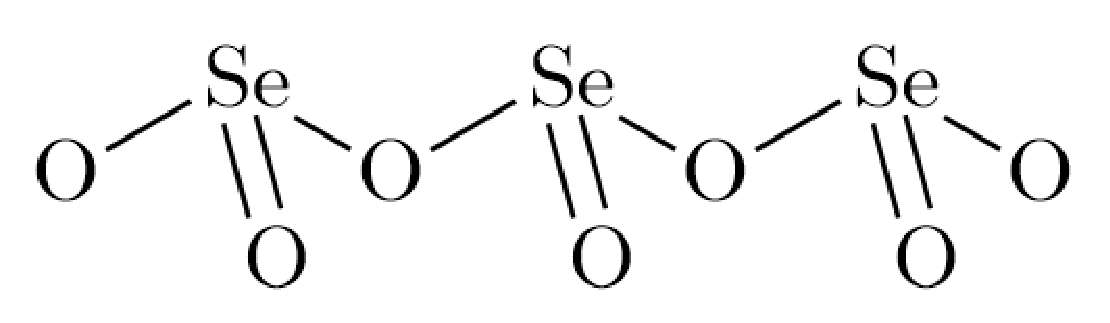
\includegraphics[scale=0.25]{picture/SeO2.eps}
    \caption{固态\ce{SeO2}的长链结构}
\end{figure}
\begin{substance}[\ce{TeO2}]
    二氧化碲,化学式为\ce{TeO2}.固体具有两种晶型:黄色的黄碲矿$\beta$-\ce{TeO2}和白色的副黄碲矿$\alpha$-\ce{TeO2}.\ce{TeO2}在$733\tccentigrade$熔化为红色液体.\ce{TeO2}极易溶于水形成亚碲酸\ce{H2TeO3}.
\end{substance}
自然界中的\ce{TeO2}以$\beta$-\ce{TeO2}的形式存在,其中有复杂的二维层状结构,如下图所示.
\begin{figure}[H]
    \centering
    \subfigure[$\beta$-\ce{TeO2}沿$a$轴的投影图]
    {
        \begin{minipage}[b]{.45\linewidth}
            \centering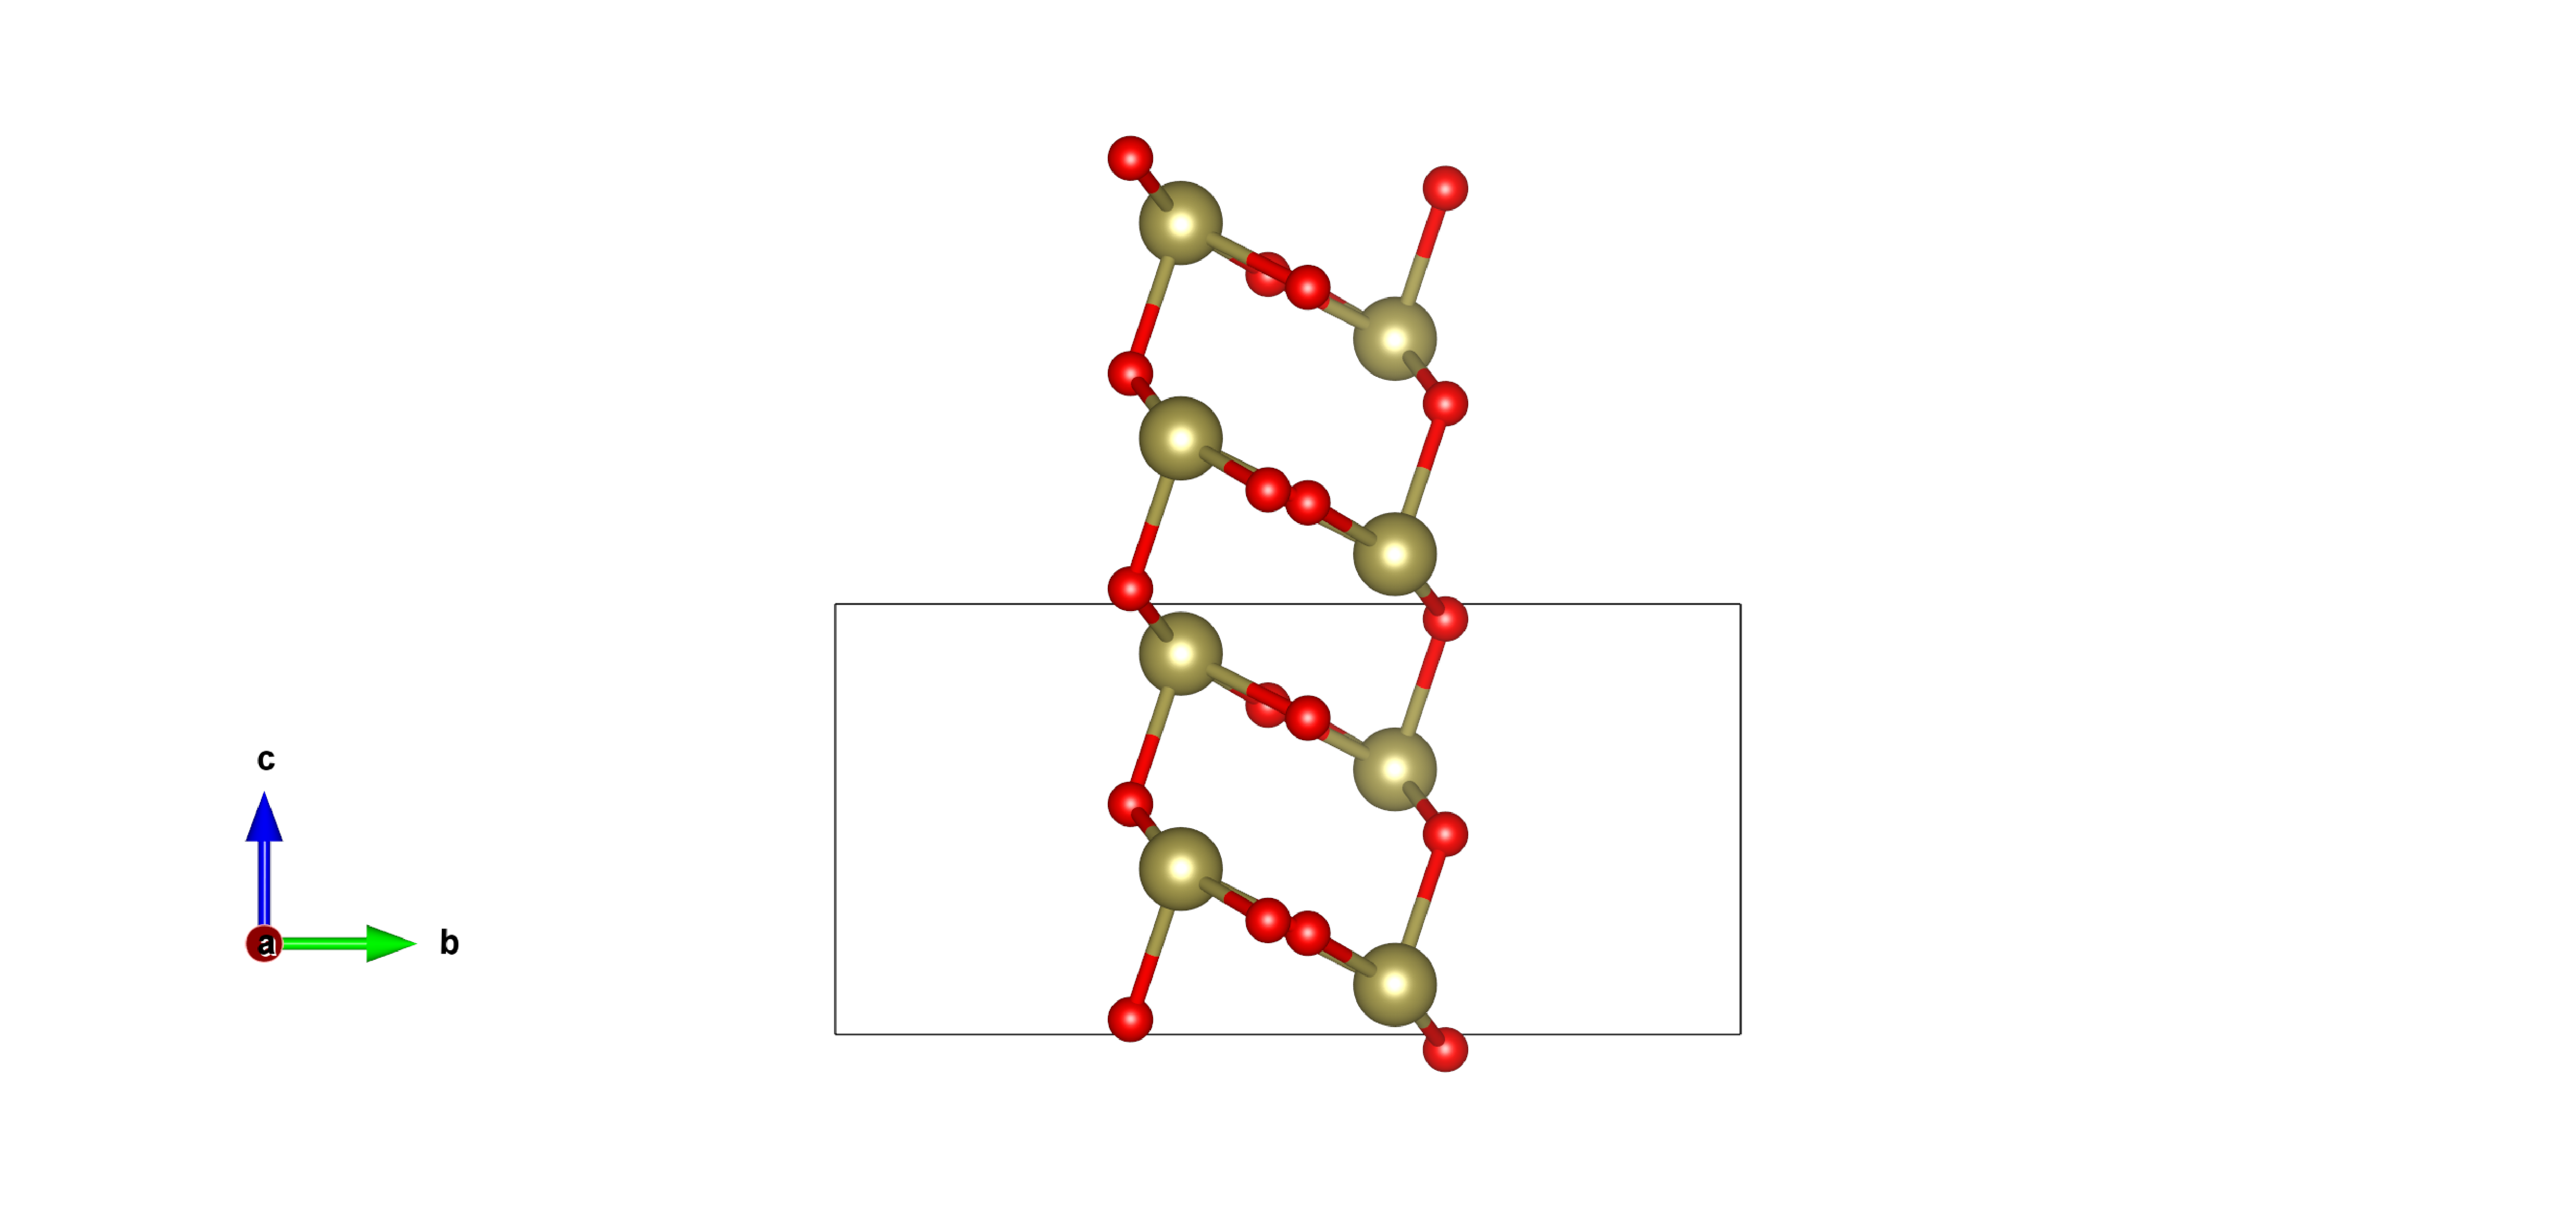
\includegraphics[scale=0.125]{picture/beta-TeO2-a.eps}
        \end{minipage}
    }
    \subfigure[$\beta$-\ce{TeO2}沿$b$轴的投影图]
    {
        \begin{minipage}[b]{.45\linewidth}
            \centering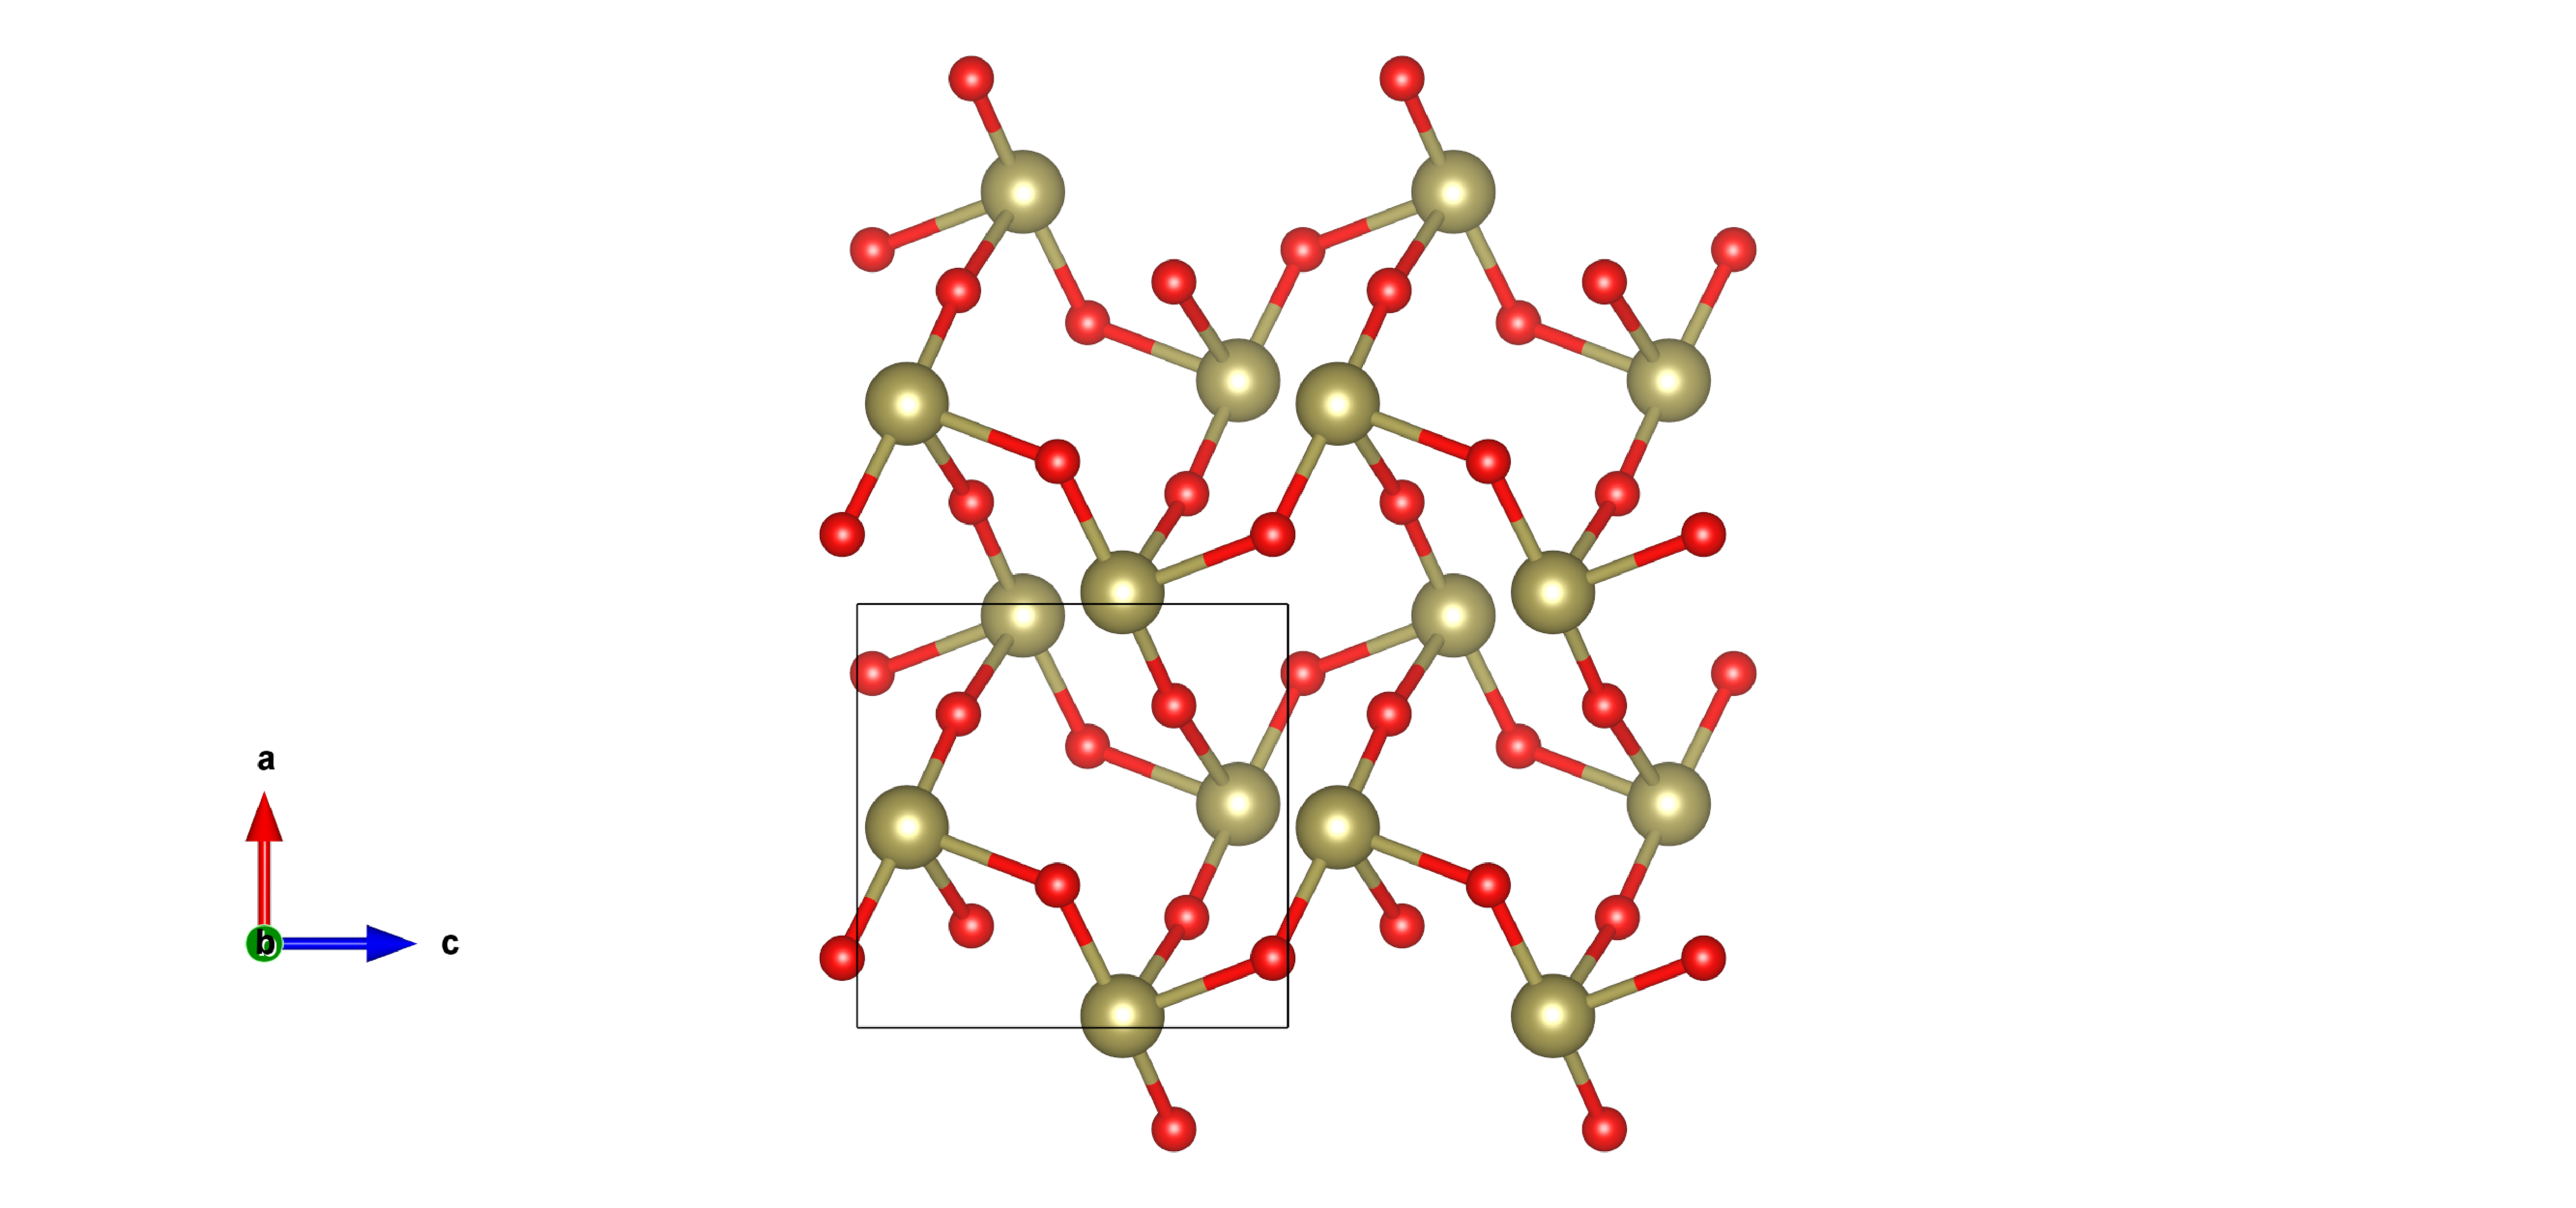
\includegraphics[scale=0.125]{picture/beta-TeO2-b.eps}
        \end{minipage}
    }
    \caption{$\beta$-\ce{TeO2}的晶体结构}
\end{figure}
而$\alpha$-\ce{TeO2}则在实验室中合成,为似金红石结构.
\paragraph{含氧酸}
与对应的氧化物相比,两种元素的$+4$价含氧酸,亚硒酸\ce{H2SeO3}和亚碲酸\ce{H2TeO3},则显得有些乏善可陈.两者均为白色的晶型固体,容易脱水成对应的氧化物.\\
\indent \ce{H2SeO3}最佳的制备方法是\ce{SeO2}水溶液缓慢结晶,或者用稀\ce{HNO3}氧化\ce{Se}粉而得到:
\begin{center}
    \ce{3Se + 4HNO3 + H2O -> 2H2SeO3 + 4NO}
\end{center}而\ce{H2TeO3}则可以由碲的四卤化物水解得到.\\
\indent \ce{H2SeO3}和\ce{H2TeO3}都是二元中强酸.
\subsubsection{\ce{Se,Te}的$\mbf{+6}$价化合物:氧化物和含氧酸}
\paragraph{氧化物}
\ce{SeO3}和\ce{TeO3}具有比较明显的区别.
\begin{substance}[\ce{SeO3}]
    三氧化硒,化学式为\ce{SeO3},是白色吸湿性的固体,在$118\tccentigrade$熔融,容易升华,在$165\tccentigrade$以上分解.
\end{substance}
由于次级周期性的缘故,将\ce{Se}氧化到$+6$价是困难的.对于\ce{S},\ce{Se}和\ce{Te}而言,只有\ce{SeO2}被氧化为\ce{SeO3}吸热:
\begin{center}
    \ce{2SeO2(s) + O2(g) -> 2SeO3(s)}\ \ \ $\Delta H_\text{m}^\ominus=+92\kJm$
\end{center}
因此,最好通过\ce{K2SeO4}与\ce{SO3}的反应制备\ce{SeO3}:
\begin{center}
    \ce{K2SeO4 + SO3 -> SeO3 + K2SO4}
\end{center}
固态的\ce{SeO3}以环状四聚体\ce{Se4O12}的形式存在,其结构示意如下.
\begin{figure}[H]
    \centering\includegraphics{picture/SeO3.eps}
    \caption{环状四聚体\ce{Se4O12}的结构}
\end{figure}
\begin{substance}[\ce{TeO3}]
    三氧化碲,化学式为\ce{TeO3}.固体具有两种晶型:橙黄色的$\alpha$-\ce{TeO3}和灰色的$\beta$-\ce{TeO3}.
\end{substance}
与\ce{SeO3}不同,\ce{TeO3}不与水作用,自身反应性也较差.
\paragraph{含氧酸}
同样地,$+6$价的\ce{Se}和\ce{Te}的含氧酸也具有比较明显的区别.
\begin{substance}[\ce{H2SeO4}]
    硒酸,化学式为\ce{H2SeO4}.无水\ce{H2SeO4}同浓硫酸的物理性质相似,有强烈的吸湿性,在水中的溶解度很大.
\end{substance}
\ce{H2SeO4}在很多方面与\ce{H2SO4}相似:\ce{H2SeO4}的$K_{\text a1}$很大,而$K_{\text a2}=1.2\times10^{-2}$亦与\ce{H2SO4}相近;硒酸盐与硫酸盐相似,这二类盐都生成一系列矾类;$\ce{Se}^{\ce{VI}}$也能生成多聚的酸\ce{H2Se2O7}等.但与\ce{H2SO4}不同的是,\ce{H2SeO4}是很强的氧化剂,甚至能溶解\ce{Au},\ce{Pd}等惰性金属.\\
\indent 可以通过各类氧化剂氧化\ce{H2SeO3}制备\ce{H2SeO4},例如:
\begin{center}
    \ce{5H2SeO3 + 2HClO3 -> 5H2SeO4 + Cl2 + H2O}
\end{center}
等等.\\
\indent $\ce{Te}^{\ce{VI}}$的含氧酸主要是原碲酸\ce{H6TeO6}.
\begin{substance}[\ce{H6TeO6}]
    原碲酸,化学式为\ce{H6TeO6},白色固体,熔点$136\tccentigrade$.
\end{substance}
原碲酸的晶体结构是由正八面体的\ce{Te(OH)6}分子构成,在溶液中也是如此.与\ce{H2SO4}或\ce{H2SeO4}不同,\ce{H6TeO6}是弱酸,其$K_{\text a1}=2\times10^{-8}$.\\
\indent \ce{H6TeO6}可以由氧化剂氧化\ce{Te}或\ce{TeO2}制备.同时,\ce{H6TeO6}也是一种中等强度的氧化剂.
\end{document}